% !TEX root = main.tex
% !TEX program = pdflatex

\documentclass[portugues]{automatex}

\title{Desenvolvimento de plataforma robótica omnidirecional}
\shorttitle{Robô móvel omnidirecional}
\author{Emílio Dolgener Cantú}
\supervisor{Eduardo Perondi}

\newacronym{rpi}{RPi}{\emph{Raspberry Pi}, computador embarcado}
\newacronym{imu}{IMU}{\emph{Inertial Measurement Unit}, ou Unidade de Medidas Inerciais}
\newacronym{pid}{PID}{Controlador Proporcional-Integral-Derivativo}
\newacronym{pi}{PI}{Controlador Proporcional-Integral}
\newacronym{tomr}{TOMR}{\emph{Three-wheeld Omnidirectional Mobile Robot}, ou Robô Móvel Omnidirecional de Três Rodas}
\newacronym{ins}{INS}{\emph{Inertial Navigation System}, ou Sistema de Navegação Inercial}
\newacronym{pkm}{PKM}{\emph{Posture Kinematic Model}, ou Modelo Cinemático de Postura}
\newacronym{ckm}{CKM}{\emph{Configuration Kinematic Model}, ou Modelo Cinemático de Configuração}
\newacronym{cdm}{CDM}{\emph{Configuration Dynamic Model}, ou Modelo Dinâmico de Configuração}
\newacronym{pdm}{PDM}{\emph{Posture Dynamic Model}, ou Modelo Dinâmico de Postura}
\newacronym{i2c}{I2C}{\emph{Inter-Integrated Circuit}, ou Circuito Inter-Integrado}
\newacronym{arm}{ARM}{\emph{Advanced RISC Machine}}
\newacronym{gpio}{GPIO}{\emph{General Purpose Input/Output}}

% Símbolos:
\newglossaryentry{angvel}{
  name = $\omega$ ,
  description = Velocidade ângular,
}
\newglossaryentry{vx}{
  name = ${v_x}$ ,
  description = Velocidade linear no eixo X do sistema de coordenadas cartesiano,
}
\newglossaryentry{vy}{
  name = ${v_y}$,
  description = Velocidade linear no eixo Y do sistema de coordenadas cartesiano,
}
\newglossaryentry{deltam}{
  name = $\delta_m$,
  description = Grau de mobilidade,
}
\newglossaryentry{deltas}{
  name = $\delta_s$,
  description = Grau de dirigibilidade,
}
\newglossaryentry{velw}{
  name =$\phi_i$,
  description = Velocidade angular da roda \emph{i},
}
\newglossaryentry{raio}{
  name = $r$,
  description = Raio das rodas utilizadas,
}
\newglossaryentry{Raio}{
  name = $R$,
  description = Distância de cada roda até o centro geométrico da estrutura,
}

\agradecimentos{Agradeço a todo mundo que ajudou.}

\resumo{O presente trabalho apresenta a implementação de uma base robótica omnidirecional holonômica, utilizando 3 omniwheels. Foram implementados um sistema de controle e um método de odometria em malha aberta. Os resultados foram xxxx.}
\myabstract{This work shows the implementation of a holonomic omnidirectional robotic platform, using 3 omniwheels. Were also implemented a control system and a method for open loop odometry. As a result, xxxx.}

\begin{document}

\maketitle % TODO: tem como dispensar esse comando, tipo redefinindo o ambiente "document"

%%%%%%%%%%%%%%%%%%%%%%%%%%%%
%% Início do documento
%%%%%%%%%%%%%%%%%%%%%%%%%%%%

%% Trabalho principal
\section{Introdução}

%\subsection{Motivação}

O interesse na área da robótica se dá pela multi-disciplinaridade do tema, que abrange um espectro de conhecimentos que vai desde mecânica estrutural até a aplicação de teorias de controle sofisticadas. A área ainda se extende por eletrônica, elétrica, computação e até mesmo psicologia. Assim, considera-se que esta área é bastante adequada a um trabalho de conclusão de um curso igualmente abrangente, que é a Engenharia de Controle e Automação.

Em aplicações industriais, a maioria dos robôs utilizados são manipuladores, que realizam tarefas repetitivas -- como soldagem ou montagem de peças -- com precisão e rapidez adequados a cada aplicação. Estes robôs, no entanto, são em geral fixos, e daí surge o estudo da robótica móvel: como um robô pode se mover sem supervisão e interagir com o mundo real? (\cite{siegwart2011introduction}) Além do interesse acadêmico, existe um significativo interesse comercial, visto que o mercado de robôs móveis, que estava em torno de 4,5 bilhões de dólares americanos em 2014, tende a duplicar até 2020 (\cite{marketsmarkets}).

\begin{figure}[h]
  \centering
  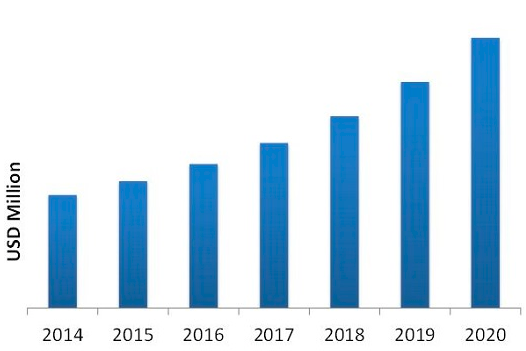
\includegraphics[width = 0.5\textwidth]{imagens/markets}
  \caption{Projeção de crescimento do mercado de robótica móvel até 2020.}
  \label{fig:markets}
  \source{\cite{marketsmarkets}}
\end{figure}

Segundo \cite{lynch2017modern}, robôs móveis são divididos em robôs não-holonômicos e robôs omnidirecionais, com diferenças significativas em planejamento de trajetória, controle e modelagem dos dois tipos de robô. Diante da natureza do presente trabalho de conclusão de curso, o escopo foi definido no âmbito dos robôs holonômicos omnidirecionais, que se destacam comercialmente pela habilidade de realizar transporte de cargas pequenas em espaços confinados -- como corredores de hospital e depósitos de armazenamento que buscam o aumento da capacidade sem perder agilidade logística nem aumentar o espaço necessário nas instalações. Academicamente, o controle de rodas omnidirecionais apresenta diversos problemas interessantes, vários dos quais serão descritos ao longo do presente trabalho. O desenvolvimento de uma plataforma robótica omnidirecional holonômica se torna útil para futuras aplicações em diversas áreas de investigação em robótica, controle e automação.

%\subsection{Descrição do Trabalho}

O presente trabalho consiste no desenvolvimento (tanto teórico quanto experimental) de uma plataforma robótica que possa se movimentar de maneira autônoma em qualquer direção do plano sem necessidade de reorientação -- apresentando holonomicidade. Após uma avaliação na bibliografia sobre os tipos de robôs factíveis de serem construídos no tempo previsto com os recursos financeiros disponíveis, optou-se pela seguinte configuração. A plataforma considerada mais adequada utiliza 3 \emph{omniwheels}, cada uma acionada por um motor elétrico dedicado, conforme o modelo mostrado na Figura \ref{fig:tomr_ritter}. Como as rodas são montadas de maneira fixa no chassi, este tipo de robô ainda oferece a vantagem de ser construído com uma estrutura mecânica mais simples, como mencionado por \cite{siciliano2016springer}. As rodas omnidirecionais utilizadas podem ser vistas em detalhe na Figura \ref{fig:omniwheel}. O sistema de movimentação é controlado por software processado em um computador embarcado a partir dos sinais fornecidos por sensores inerciais e de odometria.

\begin{figure}[h]
  \centering
  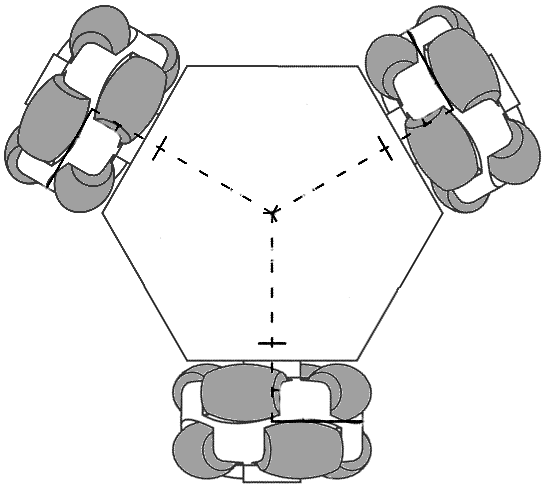
\includegraphics[width = 0.45\textwidth]{imagens/tomr_ritter_mod}
  \caption{Diagrama de um robô móvel com três rodas omnidirecionais.}
  \label{fig:tomr_ritter}
  \source{adaptado de \cite{ritter2016modelagem}}
\end{figure}

\begin{figure}[h]
  \centering
  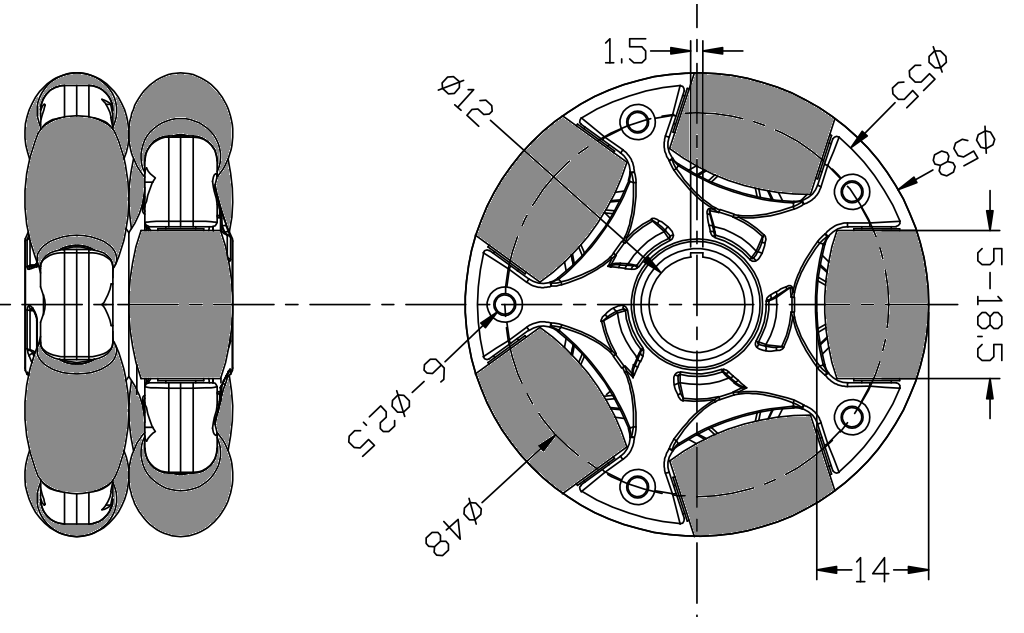
\includegraphics[width = 0.45\textwidth]{imagens/omniwheel}
  \caption{Desenho de uma roda omnidirecional.}
  \label{fig:omniwheel}
  \source{adaptado de \cite{omniwheel}}
\end{figure}

%\subsection{Objetivos}

Este trabalho tem como \textbf{objetivo geral} projetar, construir, colocar em operação e testar uma plataforma robótica omnidirecional de baixo custo, mas com características semelhantes às dos sistemas comerciais. Para atingir esse objetivo, se devem alcançar os seguintes \textbf{objetivos específicos}:

\begin{itemize}
  \item{Modelagem do robô;} %especificar se é cinemática ou dinâmica
  \item{Especificação e construção de um protótipo;}
  \item{Implantação de um algoritmo de controle;} % eu tinha colocado implementação, mas perondi pediu implantação
  \item{Implantação de instrumentação e algoritmo de localização;}
  \item{Realizar experimentos de seguimento de trajetórias e analisar os resultados obtidos.}
\end{itemize}

%\subsection{Organização do Trabalho}

O trabalho está organizado da seguinte maneira:
\begin{itemize}
  \item{Na \hyperref[sec:revbib]{Seção 2}, é apresentada a revisão bibliográfica, versando sobre robótica móvel, técnicas de controle utilizadas na área e um breve resumo sobre métodos de localização, além de uma exposição dos trabalhos mais recentes envolvendo robôs omnidirecionais;} %colocar planejamento de trajetória e hardware tbm??
  \item{Na \hyperref[sec:montagem]{Seção 3}, especificação do hardware, estrutura mecânica e montagem do protótipo;}
  \item{Na \hyperref[sec:teorico]{Seção 4}, é apresentado o desenvolvimento teórico da modelagem do robô e dos algoritmos de controle e localização;}
  \item{Na \hyperref[sec:software]{Seção 5} são implementados os algoritmos descritos na seção anterior;}
  \item{Na \hyperref[sec:experimental]{Seção 6}, é desenvolvido e realizado um experimento para avaliar o desempenho do robô projetado;}
  \item{Por fim, na \hyperref[sec:resultados]{Seção 7}, serão apresentados as análises e discussões sobre os resultados dos experimentos, a conclusão sobre o trabalho como um todo e algumas propostas para futuros trabalhos.}
  \item{VERIFICAR. TEM UMA SESSÃO A MAIS AQUI.. DE ONDE SAIU \textbf{CONCLUSÃO VS RESULTADOS}}
\end{itemize}

Além do descrito, o trabalho ainda contém os seguintes apêndices:
\begin{itemize}
  \item{\hyperref[sec:custo]{Apêndice A}, da descrição dos custos do projeto;}
  \item{o q mais vier.}
\end{itemize}

\section{Revisão Bibliográfica}
\label{sec:revbib}

\subsection{Fundamentação Teórica}

% modelagem
Para que se possa compreender o comportamento de um robô e desenvolver aplicações, é necessário obter o modelo de tal robô. Para robôs móveis, em contraste com braços robóticos, por exemplo, há um nível de complexidade adicional na estimação da posição do robô, visto que a plataforma móvel não possui nenhuma extremidade fixa em um ponto conhecido. No caso do robô omnidirecional com 3 rodas, se deseja obter um \textbf{modelo cinemático} que relacione as velocidades de cada roda à posição do robô no ambiente. Para robôs móveis em geral, primeiro se deve analisar as restrições de movimento adicionadas ao sistema por cada roda. Ao se utilisar rodas omnidirecionais, tais restrições não existem, simplificando a obtenção da cinemática direta do TOMR. Tal análise é demonstrada por diversos autores, como \cite{siegwart2011introduction}, por exemplo, e será utilizada nas próximas seções. Ainda de acordo com os autores, conforme a velocidade de operação aumenta, se torna importante realizar a análise dos efeitos dinâmicos do sistema -- massa e força -- durante a implantação. A \textbf{modelagem dinâmica} do robô em questão ainda é discutida, variando conforme a aplicação desejada, sendo uma das opções apresentada por \cite{kim2014minenergy}.

% planejamento de trajetória:
Também são apresentados por \cite{lynch2017modern} diversos métodos de \textbf{planejamento de trajetória} para robôs, ou seja, a maneira como o robô (ou um efetuador) se movimenta de um determinado ponto até outro. Há diversos métodos de se implantar trajetórias, com diversos níveis de complexidade computacional. Implementações mais simples podem ser uma linha reta de um ponto a outro, com atuação repentina, causando picos de aceleração, ou mais refinadas, realizado interpolações polinomiais de quinta ordem para garantir velocidades e acelerações nulas nos pontos de origem e destino. Também é importante analisar o perfil de velocidade executado pelo robô, para garantir a operação mais eficiente possível para as características dinâmicas de cada aplicação.

% controle
Segundo \cite{lynch2017modern}, aplicar controle com realimentação em robôs omnidirecionais é relativamente simples, visto que esse tipo de plataforma robótica apresenta controlabilidade -- ou seja, sempre há um conjunto de velocidades \textbf{$\dot\phi$} para as rodas que ocasiona numa certa velocidade \textbf{$v$} (translacional e rotacional) para o robô. \cite{siegwart2011introduction} sugerem a utilização de um controlador com realimentação de estados. Neste paradigma, o algoritmo de geração de trajetória divide o caminho a ser percorrido em diversos pontos, e o controlador implementado garante que o robô percorra tal trajeto, como se os dois sistemas -- planejamento de trajetória e controle --, estivessem operando em camadas hierárquicas.

A maioria dos autores se concentra em controladores que levam em consideração apenas a modelagem cinemática do sistema. No entanto, nos casos em que o modelo do robô exija considerações dinâmicas e não-lineares, controladores mais complexos são utilizados. Dentre outros, \cite{siciliano2016springer} descrevem o método de controle por torque computado, bastante popular, no qual o modelo dinâmico inverso é utilizado para linearizar a malha de controle. Ainda, conforme \cite{indiveri2009swedish}, o controle por torque computador configura um sistema de controle centralizado, enquanto a utilização de um PID para cada roda seria um exemplo de controle descentralizado.

%odometria
A localização do robô no ambiente é essencial para o bom funcionamento de um robô móvel. Conforme \cite{lynch2017modern}, se realiza \textbf{odometria} -- a medição da distância percorrida -- atrávés da integração das velocidades das rodas. Como o sensoriamento das rodas é muito comum, através de \textit{encoders} de quadratura, por exemplo, tornando a odometria algo barato e conveniente. No entanto, devido às sucessivas integrações realizadas, erros de estimação tendem a se acumular ao longo do tempo de operação, devido a deslizamentos das rodas e erros numéricos, principalmente. Sensores relativos como acelerômetros e giroscópios também tendem a acumular o mesmo tipo de erro. Assim, conforme \cite{siegwart2011introduction}, se recomenda utilizar métodos de localização absolutos de tempo em tempo, como magnetômetros, GPS e marcadores fixos no ambiente, ou, conforme complementado por \cite{lynch2017modern}, se pode realizar uma integração das leituras de diversos sensores. Esse método é chamado de \textbf{fusão de dados}.

%Caso necessário, capítulo 35 de \cite{siegwart2011introduction}: Sensor Data Fusion.

%implantação
\cite{siciliano2016springer}: Capítulo 12, Arquitetura de sistemas robóticos.

\cite{craig2017introduction}: pg 350, chapter 12 -> linguagens de programação para robótica

O \textbf{Raspberry Pi} é um \emph{single board computer}, que utiliza a arquitetura \acrshort{arm} em seu processador, ideal para dispositivos alimentados por baterias por consumir pouca energia e gerar pouco calor. O processador possui quatro núcleos, e um \emph{clock} de 1,2 GHz -- poder computacional equivalente há um computador de mesa comum. O \acrshort{rpi} utiliza um sistema operacional GNU/Linux, e \emph{software} deve ser desenvolvido para ser executado nesta plataforma. Há ainda 40 pinos de \acrshort{gpio} que podem ser utilizados para conectar sensores, atuadores e diversos componentes, e suporte nativo a \acrshort{i2c} (\cite{upton2014raspberry}).

% Software, implementação
% - tempo de ciclo
% - real-time
% - protocolos de comunicação

Para a comunicação dos periféricos com este computador, é necessário utilizar algum protocolo de comunicação. O protocolo \textbf{\acrlong{i2c}}, é geralmente utilizado em robôs, csom um grande suporte tanto pela \acrshort{rpi} (\cite{upton2014raspberry}) quanto pelos componentes em geral utilizados (\cite{MPU6050} e a bússola e o arduino se eu usar). Com este protocolo, descrito em \cite{semiconductors2000i2c}, dados podem ser transmitidos a 100 Kbps -- ou 400 Kbps quando utilizado o \emph{fast mode}. São utilizados duas linhas bidirecionais no barramento: SDA para os dados e SCL para os sinais de \emph{clock}. O número de dispositivos conectados ao barramento só depende do limite de capacitância descrito na especificação. Resistores de \emph{pull-up} são necessários para manter a linha em estado lógico alto quando não utilizada, porém estes resistores estão presentes internamente no \emph{Raspberry Pi}, por exemplo.

ARDUINO? TEMPO REAL?

\subsection{Estado da Arte}

%% RODAS

A grande maioria dos robôs construídos com \textbf{\emph{omniwheels}} utiliza 3 rodas em uma configuração triangular simétrica -- como apresentado na Figura \ref{fig:tomr_ritter} --, a exemplo de \cite{ritter2016modelagem}, \cite{samani2007comprehensive}, \cite{williams2002dynamic} e \cite{indiveri2009swedish}, entre outros. Alguns autores, como \cite{krinkin2015design} e \cite{rojas2006holonomic} utilizam 4 rodas, sendo que este último desenvolveu algoritmos para que o robô continuasse operando mesmo que um dos motores deixe de funcionar. Em diversos trabalhos existe uma preocupação em relação a possíveis derrapagens das rodas ao aumentar a velocidade de operação. \cite{williams2002dynamic} apresentam um estudo sobre os coeficientes de atrito de rodas omnidirecionais em diversas superfícies e um modelo dinâmico que leva tal efeito em consideração. \cite{samani2007comprehensive} utilizam 3 rodas motrizes e outras 3 rodas livres ligadas a \textit{encoders}, para que deslizamentos devido a torque excessivo não afetem a odometria.

\cite{jung2001fault} construíram um robô omnidirecional e um sistema de transmissão mecânica que permite holonomicidade utilizando rodas convencionais. Sugerem ainda modos de operação para o robô caso algum dos motores parem de funcionar, passando a se comportar de maneira similar a um robô diferencial. Nestes casos de falha, no entanto, se perde a capacidade omnidirecional.

%% MODELAGEM e CONTROLE
Há muitas técnicas de \textbf{controle} desenvolvidas para estes sistemas. Assim, é possível que cada autor utilize a que mais convenha às suas necessidades específicas. \cite{ritter2016modelagem} utiliza um controlador PID para cada roda, com parâmetros escolhidos empiricamente. Por sua vez, o robô torna-se difícil de controlar com velocidades acima de 1 m/s, segundo resultados de simulações. \cite{samani2007comprehensive} utilizam 3 PID, para controlar posição e orientação do robô, e relatam em detalhes o desenvolvimento de tais controladores. Em contraste, \cite{rojas2006holonomic} e \cite{indiveri2009swedish} também utilizam PID, porém para o controle de individual de cada motor, utilizando apenas o modelo cinemático do sistema. \cite{indiveri2009swedish} também sugere estratégias para evitar saturação dos atuadores.

Tanto \cite{treesatayapun2011discrete} quanto \cite{oubbati2005velocity} utilizam redes neurais para ajustar parâmetros dos controladores, sendo que no primeiro se tem uma estrutura de controle baseada em redes neurais enquanto que no segundo se utilizam as redes para calcular os parâmetros de 5 controladores PID, melhorando o desempenho mesmo levando em consideração de não-linearidades nos modelos dinâmicos utilizados. \cite{oubbati2005velocity} ainda mencionam que os resultados obtidos não foram os melhores possíveis, devido à dificuldade de se coletar dados de treinamento para as redes.

%% ODOMETRIA:
A maioria das implementações de robôs móveis hoje em dia combinam diversas técnicas de \textbf{localização e odometria} para implantar a realimentação necessária aos sistemas de controle. \cite{ginzburg2013indoor} propõem um sistema de localização para robô omnidirecional baseado em odometria (localização relativa) e triangulação ativa de sensores no ambiente (localização absoluta), com fusão de dados para obter o resultado final. \cite{rojas2006holonomic} utilizam a leitura dos \emph{encoders} das rodas e uma câmera externa, enquanto que \cite{garcia2015gyro} utilizam apenas um giroscópio e um sensor de distância. \cite{rohrig2010laser}, por outro lado, utilizam medições de distância utilizando sensores laser em AGV.

\cite{lowcostIMU} mostram que é possível executar um algoritmo de determinação de atitude a partir de uma IMU utilizando TRIAD, filtros de Kalman, covariância de Allen e a plataforma Arduino UNO, com razoável precisão. \cite{park1996dead} também analisam fusão de dados utilizando um filtro de Kalman indireto para realizar \emph{dead-reckoning} a partir da leitura de \emph{encoders} e um giroscópio. Métodos de localização também são desenvolvidos em outras áreas, como relata \cite{jimenez2009comparison}, que implementam três métodos de localização baseados em INS para trajetórias de pedestres, concluindo que os resultados podem ser melhorados quando há mais qualidade na detecção da orientação. \cite{steinhoff2010pocket} obtiveram resultados similares na mesma área.

%% SOFTWARE
Dos trabalhos mencionados, poucos entram em detalhes quanto ao \emph{hardware} utilizado. \cite{oubbati2005velocity} utilizam um computador embarcado de 2,6 GHz, uma grande evolução em relação a \cite{feng1989servo}, que utilizavam um computador Motorola 68000 com aproximadamente um milésimo da capacidade computacional daquele. \cite{takemura2007development} e \cite{loh2003mechatronics} utilizam computadores externos, envolvendo atrasos na comunicação entre tais computadores e o robô. \cite{lowcostIMU} apresentam um sistema que implementa um filtro de Kalman em um microprocessador Arduino UNO, uma alternativa de baixo custo. Diversos trabalhos mais recentes, como \cite{krinkin2015design}, utilizam especificamente o computador embarcado \textbf{Raspberry Pi} para o processamento e um \textbf{Arduino} para a interface com sensores e atuadores -- solução esta também adotada neste trabalho.

%% TESTES
Para a avaliação dos resultados da plataforma construída, \cite{loh2003mechatronics} implementaram 4 tipos de trajetória: translação retilínea , translação curvilínea -- ambas sem alteração na orientação --, rotação pura e um caminho combinado de rotação em torno do seu centro e translação retilínia em relação às referências globais. Duas canetas foram montadas no robô, uma no centro e outra na periferia, para avaliar o resultado das movimentações executadas.

% !TEX root = main.tex
% !TEX program = pdflatex


\section{Especificação e montagem do protótipo}
\label{sec:montagem}

Conforme mencionado nas seções anteriores, o robô construído possui três rodas em uma configuração simétrica. Apesar da falta de redundância -- pois se alguma das rodas falhar se perde a holonomicidade --, robôs omnidirecionais com 3 rodas (TOMR) são utilizados com mais frequência por serem mais simples de se implementar, apresentarem custo mais baixo (pois motores e rodas são responsáveis por 53\% do custo do projeto, conforme o \hyperref[sec:custo]{Apêndice A}), e uma certa economia de peso.
eird since it's a conversion from a regula
As rodas utilizadas -- mostradas na Figura \ref{fig:omniwheel} --, medem 58 mm de diâmetro, com estrutura em plástico e dez roletes emborrachados, e possuem capacidade de carga nominal de 3 kg \citep{omniwheel}, suficiente para os fins de demonstração do projeto. Cada roda é acionada por um motor de corrente contínua com caixa de redução, com uma velocidade nominal no eixo de saída de 210 rpm para uma tensão de 6 V. A máxima potência do motor está especificada para uma corrente de 1,1 A, a 110 rpm. Incluso no motor está um \textit{encoder} de quadratura, que permite a leitura da velocidade da roda e da direção de rotação. Com a relação de redução, se tem que para cada revolução da roda se tem 341,2 pulsos do sensor, e portanto cada pulso representa 0.01841 radianos \citep{motor}.
%Mais info sobre a ponte H: http://linksprite.com/wiki/index.php5?title=DC_Motor_Driver_Breakout_%28L298_Chipset%29#Arduino_Sample_Code

Além da utilização dos \textit{encoders} para implementação da odometria, também foi instalada na estrutura uma bússola, para garantir uma medida absoluta da orientação do robô (sem os erros que se acumulam nos métodos de \textit{dead-reckoning}). O modelo utilizado é a HMC5883L, já instalada em uma placa com alguns componentes necessários para seu funcionamento. A precisão do circuito, de acordo com o fabricante, é de 2 graus \citep{HMC5883L}. Para complementar a odometria, também foi instalada no robô uma unidade de medidas inerciais MPU6050, que possui acelerômetro e giroscópio em torno dos três eixos utilizados \citep{MPU6050}. Os sensores descritos neste parágrafo foram adquiridos e montados à estrutura, porém não foi realizada sua implementação. Os dois periféricos utilizam o protocolo de comunicação I2C \citep{semiconductors2000i2c}, também compatível com o computador utilizado.

Foi adquirida também uma bateria com capacidade de carga de 2000 mAh e 7,2 V de tensão nominal. Ligados à bateria, se tem 3 reguladores de tensão \textit{step down} MP2307, especificados para fornecer corrente constante de 3 A cada um, suportando picos de até 4 A \citep{MP2307}. A tensão de saída dos reguladores foi configurada em 5 V (para o computador), 3,3 V (para os \textit{encoders}) e 6 V (para os motores). A bússola e a IMU tem tensão de alimentação de 3,3 V, podendo ser ligadas ao mesmo regulador que os \textit{encoders} quando forem eventualmente integradas ao sistema. Como cada motor opera em geral com correntes abaixo de 1 A, o regulador utilizado é adequado, porém apresenta margens de capacidade consideravelmente pequenas.

O acionamento dos motores se dá por um circuito de pontes H. Há duas destas placas, e cada uma pode acionar dois motores. Assim, se tem a possibilidade de utilizar mais um motor em trabalhos futuros. Os \textit{driver} são desenvolvidos em torno do circuito L298N, que pode fornecer 4 A de corrente contínua distribuída entre as cargas \citep{L298N}. O chaveamento de cada canal dos \textit{drivers} é feito por meio de modulação de largura de pulso, fornecida pelo computador. Assim como os demais componentes, os \textit{drivers} foram fornecidos integrados a uma placa montada, com terminais para fixação de cabeamento e dissipadores de calor.

Todo o processamento é realizado por um \textbf{Raspberry Pi}, um \emph{single board computer}, que utiliza a arquitetura \acrshort{arm} em seu processador, ideal para dispositivos alimentados por baterias por consumir pouca energia e gerar pouco calor. O processador possui quatro núcleos, e um \emph{clock} de 1,2 GHz -- poder computacional equivalente há um computador de mesa comum. O \acrshort{rpi} utiliza um sistema operacional GNU/Linux, e \emph{software} deve ser desenvolvido para ser executado nesta plataforma. Há ainda 40 pinos de \acrshort{gpio} que podem ser utilizados para conectar sensores, atuadores e diversos componentes, e suporte nativo a \acrshort{i2c} \citep{upton2014raspberry}.

Para unir todos os componentes descritos, se projetou uma estrutura central, como um chassi. Tal estrutura pode ser vista na Figura \ref{fig:chassi}. No centro geométrico da estrutura e na periferia, próximo a uma das rodas, foram feitos dois orifícios que devem acomodar uma caneta hidrográfica cada. Assim, durante a fase de testes, se pode acompanhar graficamente a evolução cinemática do robô. Devido a localização central de uma das canetas, todos os componentes foram instalados na periferia da estrutura. Se tomou ainda o cuidado de instalar os CI de acelerômetro e giroscópio o mais próximo ao centro possível, para que as componentes de aceleração centrípeta dos movimentos com componentes de rotação não influenciassem em demasiado nos resultados. A IMU poderia ter sido colocada no centro geométrico, e este erro poderia ser introduzido no traço da caneta. No entanto, como a odometria e localização dependem muito mais dos sensores montados nos motores do que da IMU, se preferiu manter a caneta no centro, mantendo o MPU6050 o mais próximo possível. A bússola também foi montada relativamente próxima ao centro do robô, se tomando o cuidado de alinhar os eixos dos sistemas de coordenadas dos sensores com os do robô.

\begin{figure}[h]
  \centering
  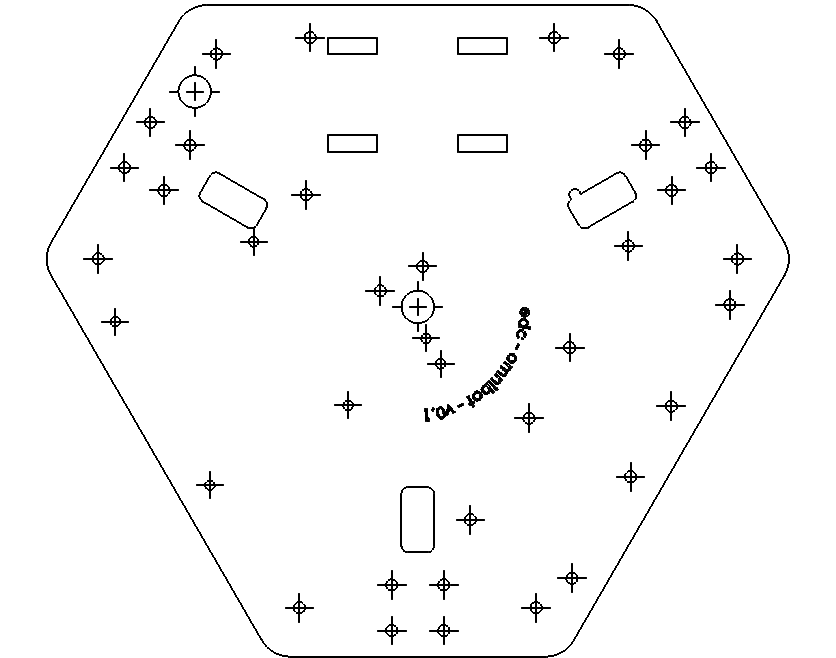
\includegraphics[width = 0.45\textwidth]{imagens/chassidxf}
  \caption{Chassi projetado.}
  \label{fig:chassi}
\end{figure}

Todos os componentes adquiridos possuem furos para fixação por meio de parafusos com 3 mm de diâmetro. A estrutura foi projetada com furos de 3,5 mm de diâmetro, para compensar possíveis erros de medição (visto que nem todos os componentes apresentaram seus desenhos nas informações técnicas) e possíveis tolerâncias de fabricação. Além dos furos de fixação dos componentes, também foram introduzidos orifícios próximos aos motores, para passagem dos cabos de um lado a outro da placa, e orifícios para fixação da bateria com presilhas plásticas. Na mesma área destinada à fixação da bateria se adicionou furação capaz de receber uma placa Arduino MEGA, caso se deseje utilizar um microcontrolador em trabalhos futuros. Também foram adicionados 6 furos na periferia do chassi, para possibilitar a montagem de outra chapa sobre a dos componentes, caso sejam realizados trabalhos que exijam a expansão da estrutura.

A plataforma projetada foi então fabricada, utilizando chapas de acrílico transparente de 5 mm de espessura. Se cogitou produzir tal estrutura em alumínio, porém se mostrou mais prático utilizar o acrílico. Entre as vantagens do material plástico se podem destacar a fácil obtenção, baixo custo, isolamento elétrico (permitindo montar os componentes eletrônicos diretamente sobre o chassi) e a possibilidade de fabricação utilizando uma máquina de corte a \textit{laser}, que elimina o limite inferior de tamanho de brocas e fresas em relação a fresadora CNC considerada originalmente. A espessura foi escolhida empiricamente, dentro das disponíveis, de maneira relativamente conservadora, e atendeu as necessidades. Na Figura \ref{fig:montagem} se pode ver a montagem final do protótipo. Os furos sobredimensionados não afetaram o alinhamento das peças.

\begin{figure}[h]
  \centering
  
\includegraphics[width = 0.45\textwidth]{imagens/edc}
  \caption{Protótipo montado, sem as canetas. TROCAR FIGURA}
  \label{fig:montagem}
\end{figure}

TERMINAR DE FALAR SOBRE AS LIGAÇÕES ELÉTRICAS QUANDO EU FIZER A LIGAÇÃO DEFINITIVA.
TERMINAR DE FALAR SOBRE AS LIGAÇÕES ELÉTRICAS QUANDO EU FIZER A LIGAÇÃO DEFINITIVA.
TERMINAR DE FALAR SOBRE AS LIGAÇÕES ELÉTRICAS QUANDO EU FIZER A LIGAÇÃO DEFINITIVA.
TERMINAR DE FALAR SOBRE AS LIGAÇÕES ELÉTRICAS QUANDO EU FIZER A LIGAÇÃO DEFINITIVA.

O custo de aquisição dos componentes relatados pode ser visto detalhado no \hyperref[sec:custo]{Apêndice A}. Cabe ressaltar que todos os itens foram comprados em dobro, para realizar a montagem de dois robôs para futuros trabalhos no LAMECC (Laboratório de Mecatrônia e Controle).

\section{Desenvolvimento Teórico}
\label{sec:teorico}

%% MODELAGEM:
%PARK: pg 468
\subsection{Modelagem Cinemática}

Primeiramente, se definem dois sistemas de coordenadas. O primeiro, $(x_I,y_I)$, é o sistema de coordenadas global, fixo no ambiente. O segundo, $(x_R,y_R)$, está centrado no próprio robô. Ainda se pode definir o ângulo $\theta$ como a orientação do robô -- ou seja, o ângulo entre os dois sistemas de coordenadas. Tal relação pode ser vista na Figura \ref{fig:ref}, e a transformação de um sistema para o outro é descrita na Equação \ref{eq:world_ref}, conforme \citet{siegwart2011introduction} e \citet{ritter2016modelagem}.

\begin{figure}[h]
  \centering
  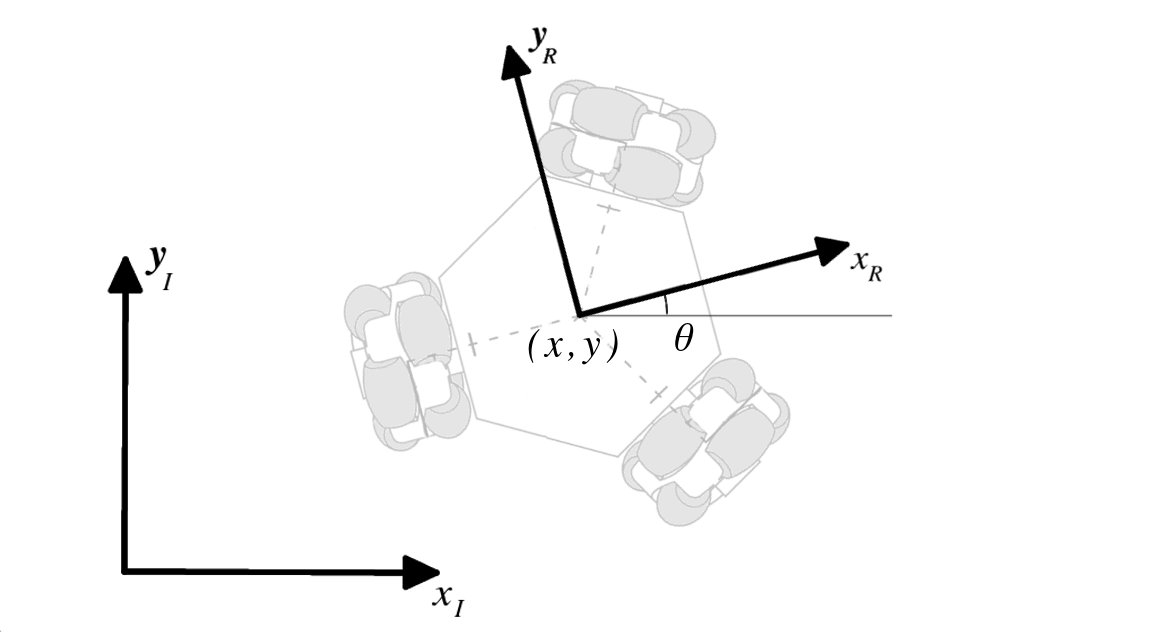
\includegraphics[width = 0.65\textwidth]{imagens/ref}
  \caption{Sistemas de coordenadas global I e relativo ao centro do robô R.}
  \source{Adaptado de \citet{ritter2016modelagem}}
  \label{fig:ref}
\end{figure}

\begin{equation}
  \begin{pmatrix}
    x_I \\
    y_I \\
    \theta
  \end{pmatrix}
  =
  \begin{pmatrix}
    cos \theta & -sen \theta & 0 \\
    sen\theta  &  cos \theta & 0 \\
    0          & 0          & 1
  \end{pmatrix}
  \begin{pmatrix}
    x_R \\
    y_R \\
    \theta
  \end{pmatrix}
  \label{eq:world_ref}
\end{equation}

O último termo da Equação \ref{eq:world_ref} também pode ser descrito como $q_R$, e o vetor de velocidades $[v_x, v_y, \omega_z]^T$, centrados no sistema de coordenadas do robô, é $\dot{q_R}$. Com o objetivo de mapear a velocidade de giro das rodas $\dot{\phi} = [\dot{\phi}_1, \dot{\phi}_2, \dot{\phi}_3]^T$ às velocidades $\dot{q_R}$, se utiliza a modelagem cinemática apresentada por \citet{siegwart2011introduction}, com as referências apresentadas na Figura \ref{fig:robo_vel}. Na figura,  A mesma modelagem é utilizada por \citet{ritter2016modelagem}, porém com outra sequência e sentido de giro para as rodas.

\begin{figure}[h]
  \centering
  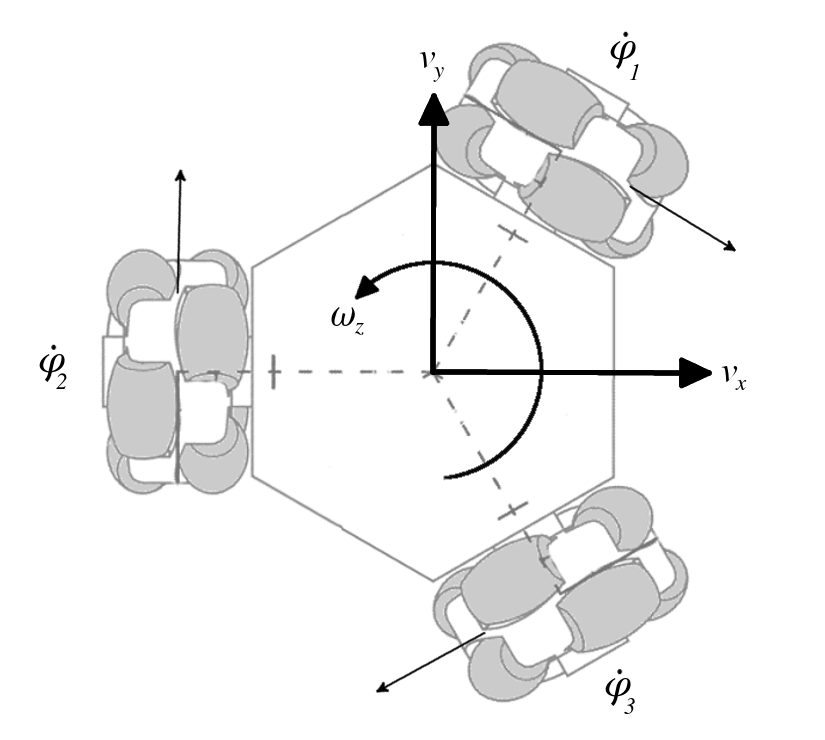
\includegraphics[width = 0.5\textwidth]{imagens/robot_vel4}
  \caption{Vista superior do robô, mostrando as convenções adotadas. As grandezas $v_x$ e $v_y$ estão no sistema de coordenadas do robô.}
  \label{fig:robo_vel}
\end{figure}

Assim, para um robô com 3 rodas dispostas em simetria radial em torno do centro da estrutura, a cinemática direta é dada pela Equação \ref{eq:dk}. Diversos autores utilizam variações da mesma modelagem (\citet{rojas2006holonomic}, \citet{pin1994new}, entre outros). Nas equações apresentadas, $r$ é o raio de cada roda e $R$ o raio do robô (a distância do centro da roda ao centro da estrutura do robô).

\begin{equation}
  \begin{pmatrix}
    v_x \\
    v_y \\
    \omega_z
  \end{pmatrix}
  =
  \frac{r}{3R}
  \begin{pmatrix}
    -\frac{3R}{\sqrt{3}} & 0   & \frac{3R}{\sqrt{3}} \\
    R                    & -2R & R                   \\
    1                    & 1   & 1
  \end{pmatrix}
  \begin{pmatrix}
    \dot{\phi_1} \\
    \dot{\phi_2} \\
    \dot{\phi_3}
  \end{pmatrix}.
  \label{eq:dk}
\end{equation}

Também se deseja utilizar a cinemática inversa do modelo, obtida realizando-se a inversão da matriz de transformação apresentada na Equação \ref{eq:dk}, é dada pela Equação \ref{eq:ik}. Nota-se que esta inversão é simplificada no caso do robô com 3 rodas, visto que quando há mais rodas é formada uma matriz $3 \times n$, sendo $n$ o número de rodas, e se deve utilizar uma matriz pseudo-inversa, conforme demonstrado por \citet{rojas2006holonomic}.

\begin{equation}
  \begin{pmatrix}
    \dot{\phi_1} \\
    \dot{\phi_2} \\
    \dot{\phi_3}
  \end{pmatrix}
  =
  \frac{1}{r}
  \begin{pmatrix}
    -\frac{\sqrt{3}}{2} & \frac{1}{2} & R \\
    0                   & -1          & R \\
    \frac{\sqrt{3}}{2}  & \frac{1}{2} & R
  \end{pmatrix}
  \begin{pmatrix}
    v_x \\
    v_y \\
    \omega_z
  \end{pmatrix}
  \label{eq:ik}
\end{equation}

Como pela classificação de \citet{campion1996structural} um \acrshort{tomr} é caracterizado na categoria (3,0), o modelo cinemático das equações \ref{eq:dk} e \ref{eq:ik} é controlável, estável e descreve a posição, orientação e suas derivadas de forma suficiente. % O modelo cinemático da Equação \ref{eq:dk} também é utilizado por \citet{rojas2006holonomic} e \citet{ritter2016modelagem}.

%% ODOMETRIA:
% lynch, pg 492 do pdf
\subsection{Odometria}

Durante a operação do robô, se torna necessário calcular a posição da estrutura. Para o cálculo da odometria, se utiliza a metodologia mostrada em \citet{lynch2017modern}. Se assume que durante um certo intervalo de tempo $\Delta t$ se tenha velocidades de rotação constantes nas rodas, o que permite considerar $\dot{\phi_i}.\Delta t = \Delta \phi_i$. Considera-se também que a unidade de tempo deste período é arbitrária, e como se deseja integrar no mesmo intervalo posteriormente, se assume um período unitário $\Delta t = 1$. Este procedimento está descrito na Equação \ref{eq:odo}, modificada a partir da Equação \ref{eq:dk}. Na prática, é fácil contar os deslocamentos angulares $\Delta \phi_i$, visto que o número de pulsos por revolução dos \textit{encoders} é determinado.

\begin{equation}
  \begin{pmatrix}
    v_x \\
    v_y \\
    \omega_z
  \end{pmatrix}
  =
  \frac{r}{3R}
  \begin{pmatrix}
    -\frac{3R}{\sqrt{3}} & 0   & \frac{3R}{\sqrt{3}} \\
    R                    & -2R & R                   \\
    1                    & 1   & 1
  \end{pmatrix}
  \begin{pmatrix}
    \Delta{\phi_1} \\
    \Delta{\phi_2} \\
    \Delta{\phi_3}
  \end{pmatrix}.
  \label{eq:odo}
\end{equation}

De posse das velocidades da plataforma durante o período de tempo unitário $\Delta t$ -- lembrando que $v_x$, $v_y$ e $\omega_z$ estão no sistema de coordenadas centrado no corpo do robô --, se deve avaliar o deslocamento em relação ao centro do robô na posição anterior. Para o caso em que $\omega_z = 0$, numa trajetória retilínea, se tem simplesmente que $\Delta q_R = \dot{q_R}$.

No entanto, quando houve mudança de orientação no período e consequentemente $\omega_z \neq 0$, se deve levar em consideração os desvios de trajetória causados por essa rotação. Assim, se obtem $\Delta q_R$ de acordo com a Equação \ref{eq:desvio} \citep{lynch2017modern}.

\begin{equation}
  \Delta q_R
  =
  \begin{pmatrix}
    \Delta x_R \\
    \Delta y_R \\
    \Delta\theta
  \end{pmatrix}
  =
  \begin{pmatrix}
    (v_x sen(\omega_z)) + v_y (cos(\omega_z) - 1)/\omega_z \\
    (v_y sen(\omega_z)) + v_x (1-cos(\omega_z)) / \omega_z \\
    \omega_z
  \end{pmatrix}
  \label{eq:desvio}
\end{equation}

Sendo $k$ o instante antes do período de tempo analisado, para se obter a nova posição $q_I$ do robô no sistema de coordenadas global se deve utilizar a rotação $R(\theta_k)$ apresentada na Equação \ref{eq:world_ref}, e atualizando os valores da última iteração conforme a Equação \ref{eq:new_odo}.

\begin{equation}
  q_{I(k+1)} = q_{I(k)} + \Delta q_I = q_{I(k)} + R(\theta_k) \Delta q_I
  \label{eq:new_odo}
\end{equation}
%\cite{samani2007comprehensive}: Adicionam um modelo de ruído dos encoders à estimativa. TIRAR OU ELABORAR?

%% PLANEJAMENTO DE TRAJETÓRIA:
\subsection{Planejamento de Trajetória}

Para o robô desenvolvido, não há a necessidade de implementar algoritmos complexos de planejamento de trajetória (detecção de obstáculos, caminhos de mínima energia, etc.). Serão abordados caminhos ``ponto a ponto'', que levam de um ponto inicial a um ponto final, ambos em repouso \citep{lynch2017modern}.

Apesar de ser uma trajetória simples, ainda se podem aplicar considerações para uma melhor operação do sistema. Uma dessas considerações é o chamado \textit{time-scaling} da trajetóra, ou seja, a geração de uma função $s(t)$ que suavize o comportamento do robô por meio de restrições em velocidades e acelerações. Na Figura \ref{fig:poly5} se pode ver uma curva de perfil de velocidade polinomial de quinta ordem, que pode garantir velocidades e acelerações nulas nos pontos de origem e destino.

\begin{figure}[h]
  \centering
  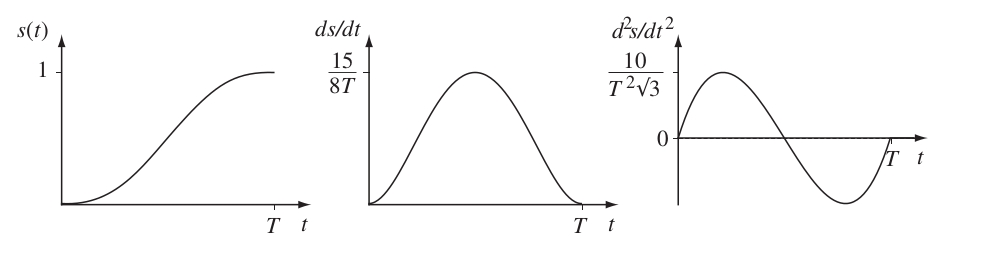
\includegraphics[width = 0.85\textwidth]{imagens/poly5}
  \caption{Deslocamento, velocidade e aceleração durante uma trajetória gerada por polinômio de quinta ordem. Aceleração e velocidade são nulas tanto no ponto de origem quanto no ponto de destino.}
  \source{\citet{lynch2017modern}}
  \label{fig:poly5}
\end{figure}

No entanto, a interpolação de um polinômio a cada cálculo de trajetória é um processo que pode envolver um certo custo computacional elevado, e devido à simplicidade dos componentes utilizados, se julgou que o aumento de suavidade na operação não fosse significativo. Portanto, neste trabalho se optou por utilizar um perfil de velocidade trapezoidal, conforme mostrado na Figura \ref{fig:trap}. Tal perfil é um dos mais comuns em robótica, devido a sua simples implementação. Os limites de aceleração foram definidos na fase de implantação do \textit{software}, de modo a evitar o deslizamento das rodas utilizadas na superfície de testes.

\begin{figure}[h]
  \centering
  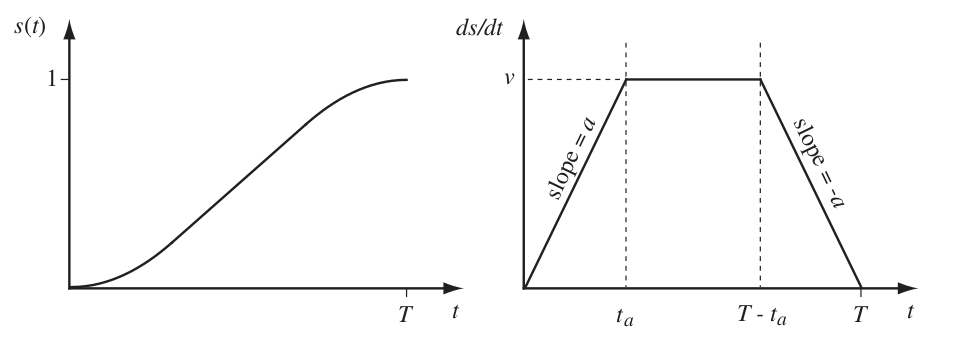
\includegraphics[width = 0.63\textwidth]{imagens/trapezoidal}
  \caption{Deslocamento e velocidade durante um deslocamento com perfil de velocidades trapezoidal. Tal perfil foi adotado neste trabalho.}
  \source{\citet{lynch2017modern}}
  \label{fig:trap}
\end{figure}

%% CONTROLE:
\subsection{Controle}

SUBSECTION EM CONSTRUÇÃO

Diversas abordagens podem ser utilizadas para a implantação de controladores em robôs omnidirecionais. Se pode realizar o controle das coordenadas desejadas, em x, y e z, ou o controle da posição de cada roda, independentemente. No caso, foram realizados três controladores de posição, em X, Y e $\omega$, utilizando a odometria discutida acima. O controlador então decide o set point de velocidade para cada roda, e envia os sinais de comando para um conjunto secundário de controladores de velocidade, 1 para cada roda. Se pode ver um esquema do sistema utilzado na FIgura \ref{fig:controle}.

\begin{figure}[h]
  \centering
  
\includegraphics[width = 0.45\textwidth]{imagens/edc}
  \caption{Arquitetura de controle utilizada.}
  %\source{\citet{lynch2017modern}}
  \label{fig:controle}
\end{figure}

Estabilidade, tipo do controle, proporcional, integral, derivativo, digital, tempo de ciclo, q q eu digo aqui, pô?

\citet{lynch2017modern}:

Loop de velocidade dentro do loop de posição. Posição das rodas ou posição em x e y e $\omega_z$?



\citet{rojas2006holonomic}: Sugerem que utilizar um controlador para cada roda é melhor do que para cada grau de liberdade. No nosso caso, é tranquilo pois temos apenas 3 rodas, mantendo o mesmo número de controladores. Devido à realimentação externa lenta, utilizam um preditor no robô. Não entram em detalhes.
motores:
https://www.banggood.com/6V-210RPM-Encoder-Motor-DC-Gear-Motor-with-Mounting-Bracket-and-Wheel-p-1044064.html?p=970719369296201312SG

Given a desired trajectory q d (t), we can adopt the feedforward plus proportional feedback linear controller (11.1) of Chapter 11 to track the trajectory: \cite{lynch2017modern}

\cite{samani2007comprehensive}: Definir os coeficientes dos PIDs é uma novela, pois devemos levar em consideração parâmetros que possuem muita variação, como o coeficiente de atrito do solo, características das baterias, entre outros. Controle deles é bem legal.
%q̇ com (t) = q̇ d (t) + K p ( q̇ d (t) − q(t)),
%(13.11)
%where K p ∈ R 3×3 is positive definite and q(t) is an estimate of the actual con-
%figuration derived from sensors. Then q̇ com (t) can be converted to commanded
%wheel driving velocities u com (t) using Equation (13.7).


%: seguimento de trajetória: malha aberta (3.6.1); Feedback (3.6.2) do livro: It is very similar to the controllers presented in [39, 100]. Others can be found in [8, 52, 53, 137]. Controle com uma matriz de ganhos K para o espaço de estados. Estável e tal. Comentam sobre camadas: planejamento -> decisão -> controlador em tempo real -> hardware.

\subsection{Limitações de Velocidade}

É importante ressaltar que toda a cinemática desenvolvida nas subseções anteriores não considera limites de velocidade para os atuadores. Numa aplicação real, entretanto, existe um ponto de saturação no acionamento de cada motor, que deve ser levada em consideração. Na Figura \ref{fig:twist_sat} se pode ver o efeito dessas limitações, conforme descrito em \citet{lynch2017modern}.

\begin{figure}[h]
  \centering
  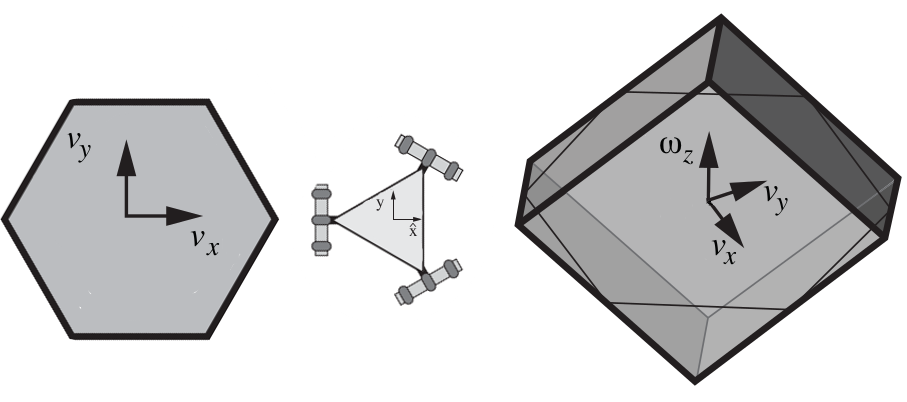
\includegraphics[width = 0.63\textwidth]{imagens/twist_sat}
  \caption{Limites de velocidade translacional e rotacional em função dos limites de saturação dos motores reais.}
  \source{Adaptado de \citet{lynch2017modern} para as coordenadas utilizadas.}
  \label{fig:twist_sat}
\end{figure}

Quando não há rotações ($\omega_z = 0$), o limite de velocidade do corpo do robô é descrito pelo hexágono mostrado na porção esquerda da Figura \ref{fig:twist_sat}: a maior velocidade possível é na direção em que uma das rodas está sendo ``arrastada'', e as componentes de velocidade das outras rodas se somam. Numa situação em que haja necessidade de rotação, a velocidade angular do robô se torna limitada da maneira mostrada no volume tridimensional à direita da Figura \ref{fig:twist_sat}, e se torna fácil enxergar que, para realizar um movimento de rotação na maior velocidade ângular possível, não se pode ter movimentos de translação, para que todos os componentes de velocidade das rodas contribuam apenas para a rotação.

Se pode dizer, então, que para aplicações reais nas quais a holonomicidade da plataforma é de fato desejável, se deve implantar um sistema de planejamento de trajetória que leve em consideração as limitações de velocidade descritas acima.

\section{Implementação dos algoritmos}
\label{sec:software}

SEÇÃO EM CONSTRUÇÃO

A implementação é difícil de encontrar nos trabalhos da bibliografia, portanto alguma coisa.

PROBLEMA: velocidade das rodas precisa o suficiente! Fazer experimentos em relação a isso.

ordem das coisas: \\
-análise dos códigos de cinemática \\
-desmembramento das funções do ritter \\
-código de acionamento dos motores \\
-bilbioteca orientada a objetos para o acionamento de cada motor e modularização do código\\
-controle de velocidade\\

Se implementou um controle proporcional simples, COLOCAR A LEI AQUI, mas se ontou que em trajetórias que necessitam do movimento das trê rodas em velocidades muito distintas se tem problemas. Para se mover em uma reta no eixo x, por exemplo, apenas as rodas 1 e 3 (verificar numeros) precisam girar, e na mesma velocidade, e fica simples de ver que o desempenho do controlador para as duas rodas vai ser similar. No entanto, na movimentação no eixo y são necessárias q a roda 1 esteja girando com o triplo da velocidade das outras duas (verificar), e assim vence a zona morta muito antes. Para solucionar isso, q q eu fáoc meu deus?\\
-implementação dos algoritmos de odometria \\
-testes para calibração dos movimentos (isso já é resultado??) \\
% 341.2/2pi pulsos/rad -> 54.3 pulsos/rad (0.01842 rad/pulso, 0.0029308323 rotações/pulso)
% VER O PAPEL NO MURAL

As equações implementadas relacionam as matrizes de transformação com a velocidade linear da periferia das rodas, $\dot{\phi}_i r$, em m/s. A leitura dos encoders é realizada em pulsos/$\mu$s. O fator de conversão aplicado é (em teoria) 534.18. Ao se utilizar o comando inverseKinematicsWorld, se obtêm as velocidades em m/s e a velocidade angular em rad/s. \\
-implementação do controle de posição \\
-algoritmo de limitação de velocidade, escalonamento \\
-organização do código \\
-interface com o usuário \\
-sequencia final de operação do código \\

O \textbf{Raspberry Pi} é um \emph{single board computer}, que utiliza a arquitetura \acrshort{arm} em seu processador, ideal para dispositivos alimentados por baterias por consumir pouca energia e gerar pouco calor. O processador possui quatro núcleos, e um \emph{clock} de 1,2 GHz -- poder computacional equivalente há um computador de mesa comum. O \acrshort{rpi} utiliza um sistema operacional GNU/Linux, e \emph{software} deve ser desenvolvido para ser executado nesta plataforma. Há ainda 40 pinos de \acrshort{gpio} que podem ser utilizados para conectar sensores, atuadores e diversos componentes, e suporte nativo a \acrshort{i2c} \citep{upton2014raspberry}.

O código de \citet{ritter2016modelagem} foi desmembrado em módulos, para separar a implementação já realizada da cinemática direta e inversa dos módulos de comunicação com o simulador utilizado. Foram escritos novos módulos para realizar a interface da Raspberry com os motores, sensores e periféricos em geral, e com essa modularidade se pode até fazer uma biblioteca para arduino blabalbalabballab, como na Figura \ref{fig:libs}.

\begin{figure}[h]
  \centering
  
\includegraphics[width = 0.45\textwidth]{imagens/edc}
  \caption{Bibliotecas utilizadas. TROCAR FIGURA}
  \label{fig:libs}
\end{figure}

Bibliotecas desenvolvidas: \\
- kinematics.h, a partir da cinemática de \cite{ritter2016modelagem}; \\
- rotary\_encoder.h, para realizar a decodificação dos encoders, desenvolvida por QUEM?? \cite{pigpio}, talvez?\\
- rpi\_interface.h, para realizar o acionamento e loops de controle para cada uma das rodas (desenvolvida pelo próprio autor);\\
- planning.h, que implementa as trajetórias de teste; \\
- user\_interface.h, que contem algumas funções básicas para conversar com o usuário, operador do sistema. IMAGINA Q MASSA UM APP C/ Bluetooth COM UM BOTÃO SÓ?

Todas as bibliotecas que utilizam entradas e saídas pelos pinos do RPi utilizam a biblioteca pigpio \citet{pigpio}, muito legalzona, até colocar nos agradecimentos.

Para calibrar o controlador em relação ao tamanho real das rodas, e obter velocidade ok, se utilizou a modelagem para definir qual deslocamento do robô, em rotação pura, necessita de 2pi rad de giro nas rodas. Foram feitos experimentos com diversos valors para calibrar isso ae.

Além de utilizar os comandos fornecidos por \citet{ritter2016modelagem}, foram implementados os modos de movimentação citados por \citet{loh2003mechatronics}: translação retilínea , translação curvilínea -- ambas sem alteração na orientação --, rotação pura e um caminho combinado de rotação em torno do seu centro e translação retilínia em relação às referências globais.

A obtenção do ângulo atual e m relação as coordenadas globais teve q ser diferente da utilizada por \citet{ritter2016modelagem}, que possuia um valor absoluto para este angulo. No caso do trablho descrito aqui, só se sabe a velocidade angular, que tambem deve ser integrada, e por isso podem aparecer mais erros.

O procedimento de opereação pode ser representado pelo diagrama apresentado na Figura \ref{fig:operation}.


\begin{figure}[h]
  \centering
  
\includegraphics[width = 0.45\textwidth]{imagens/edc}
  \caption{Fluxograma de operação do robô. TROCAR FIGURA}
  \label{fig:operation}
\end{figure}

%Para a comunicação dos periféricos com este computador, é necessário utilizar algum protocolo de comunicação. O protocolo \textbf{\acrlong{i2c}}, é geralmente utilizado em robôs, csom um grande suporte tanto pela \acrshort{rpi} (\cite{upton2014raspberry}) quanto pelos componentes em geral utilizados (\cite{MPU6050} e a bússola e o arduino se eu usar). Com este protocolo, descrito em \cite{semiconductors2000i2c}, dados podem ser transmitidos a 100 Kbps -- ou 400 Kbps quando utilizado o \emph{fast mode}. São utilizados duas linhas bidirecionais no barramento: SDA para os dados e SCL para os sinais de \emph{clock}. O número de dispositivos conectados ao barramento só depende do limite de capacitância descrito na especificação. Resistores de \emph{pull-up} são necessários para manter a linha em estado lógico alto quando não utilizada, porém estes resistores estão presentes internamente no \emph{Raspberry Pi}, por exemplo.

%O \emph{fast mode} é suportado pelo Raspberry Pi 3 B+.

Seguir o perfil de velocidade não é muito fácil, visto que dead zone. budibudibuidi \citet{indiveri2009swedish} trata saturação.

\section{Avaliação experimental}
\label{sec:experimental}

Se deseja avaliar o comportamento dos algoritmos implementados e da modelagem realizada operando o robô em três situações:
\begin{itemize}
  \item{trajetória retilínea, sem nenhum movimento de rotação, em diversas direções e com diversas velocidades de acionamento, conforme mostrado na Figura \ref{fig:reta};}
  \item{trajetória de rotação pura, analisando a variação de ângulo atingida em função do ângulo desejado e da velocidade desejada. Tal situação é ilustrada na Figura \ref{fig:giro};}
  \item{trajetória híbrida, realizando tanto uma translação retilínea arbitrária quanto uma rotação sobreposta, como no diagrama da Figura \ref{fig:hibrida}.}
\end{itemize}

\begin{figure}[h]
  \centering
  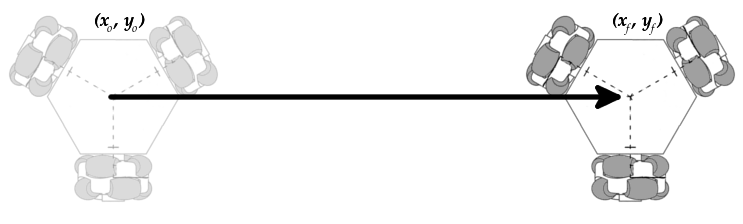
\includegraphics[width = 0.8\textwidth]{imagens/reta}
  \caption{Trajetória retilínea pura.}
  \label{fig:reta}
\end{figure}

\begin{figure}[h]
  \centering
  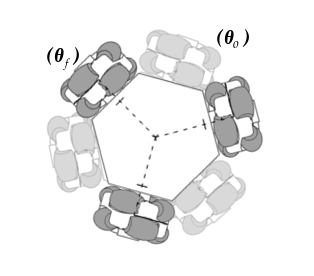
\includegraphics[width = 0.35\textwidth]{imagens/giro}
  \caption{Trajetória de giro.}
  \label{fig:giro}
\end{figure}

\begin{figure}[h]
  \centering
  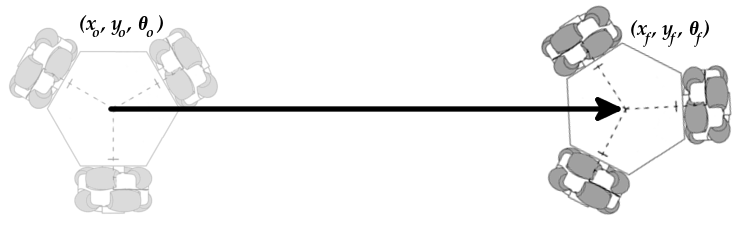
\includegraphics[width = 0.8\textwidth]{imagens/hibrida}
  \caption{Trajetória combinada.}
  \label{fig:hibrida}
\end{figure}

Se espera com a primeira trajetória, avaliar a robustez dos algoritmos quando se necessita o acionamento combinado de múltiplas rodas. Por exemplo, no eixo X, não há necessidade de movimento em uma das rodas. Em outras direções, se introduz movimentos mais lentos das rodas, o que já se viu que é um problema por causa do atrito viscoso da caixa de redução.

Com a trajetória de giro, em que as três rodas devem operar com a mesma velocidade, se deseja avaliar alguma coisa relacionada a isso. Na última trajetória, híbrida, se deseja mostrar o funcionamento do algoritmo de limitação de velocidade, e os efeitos deste fator.

Se notou que o acionamento dos motores depende de alguns fatores. Variando a frequência dos PWMs mudou o q?

O protótipo foi acionado sobre um papel enorme, com duas canetas de cores distintas instaladas nos orifícios destinados a tal.

\section{Resultados}
\label{sec:resultados}

DEVE TER EM TORNO DE DEZ PAGINAS

Desvio padrão do tmepo de execução do loop: 16,68573853

Tempo médio a cada chamada do loop de controle, em $\mu$s: 10000,03822

\section{Conclusão e Trabalhos Futuros}
\label{sec:resultados}

O trabalho apresentado neste relatório parcial conta com a introdução, revisão bibliográfica do estado da arte, revisão bibliográfica da fundamentação teórica (incompleta) e alguns comentários a respeito da modelagem que será utilizada. Todo o hardware já foi adquirido, e as próximas do trabalho são:
\begin{itemize}
  \item{fabricação do chassi do protótipo;}
  \item{finalização da revisão bibliográfica;}
  \item{modelagem do sistema;}
  \item{projeto e implantação dos controladores e métodos de odometria;}
  \item{montagem;}
  \item{experimentos e avaliações dos mesmos;}
  \item{adequação de detalhes do formato do trabalho, para que se enquadre ao modelo.}
\end{itemize}

A escrita do trabalho é realizada em paralelo ao desenvolvimento do mesmo, para melhor controle e documentação do projeto.


%% Bibliografia
\bibliography{biblio}

%% Anexos e Apêndices
\apendices
  \subsection{Custo dos componentes utilizados}
\label{sec:custo}

Há no mercado uma variada gama de componentes a serem utilizados em projetos robóticos. Para o projeto em questão, se utilizaram componentes que mostrassem um preço de mercado competitivo e grande disponibilidade. Dessa forma, se pode manter o projeto viável, mesmo que por vezes sacrificando um possível incremento de desempenho que se daria ao utilizar um componente mais robusto, por exemplo.

Na Tabela \ref{tab:custo} se pode ver a lista de componentes adquirida e os respectivos custos. Nota-se que no caso das 3 rodas há -- integrado ao valor apresentado -- as taxas de importação e conversão de moedas, visto que esses componentes foram importados dos Estados Unidos. Também é importante mencionar que o chassi foi produzido sem custo BLABLABLAB LAMECC.

\begin{table}
  \caption{Custo dos componentes utilizados no projeto.}
  \begin{tabular}{||l r c r||}
     \hline
     \textbf{Item:}   & \textbf{Valor por unidade:} & \textbf{Quantidade:} & \textbf{Valor total:} \\ \hline\hline
     Omniwheel        & R\$ 46,76                   &  3                   & R\$ 140,29            \\ \hline
     Motor c/ encoder & R\$ 119,00                  &  3                   & R\$ 357,00            \\ \hline
     Driver           & R\$ 15,00                   &  2                   & R\$ 30,00             \\ \hline
     Raspberry Pi     & R\$ 148,00                  &  1                   & R\$ 148,00            \\ \hline
     microSD 16GB     & R\$ 34,00                   &  1                   & R\$ 34,00             \\ \hline
     Arduino Mega     & R\$ 40,00                   &  1                   & R\$ 40,00             \\ \hline
     IMU MPU6050      & R\$ 9,00                    &  1                   & R\$ 9,00              \\ \hline
     Magnetômetro HMC5883 & R\$ 12,80               &  1                   & R\$ 12,80             \\ \hline
     Chassi           & R\$ 5,00                    &  1                   & R\$ 5,00              \\ \hline
     Bateria          & R\$ 120,00                  &  1                   & R\$ 120,00            \\ \hline
     Reguladores de Tensão & R\$ 4,98               &  4                   & R\$ 19,96             \\ \hline
     Parafusos        & R\$ 14,00                   &  X                   & R\$ 14,00             \\ \hline
     Diversos         & R\$ 30,00                   &  X                   & R\$ 30,00             \\ \hline\hline
                      &                             & \textbf{Custo Total:} & R\$ 946,05           \\ \hline
  \end{tabular}
  \label{tab:custo}
\end{table}

Numa escala de preços em robótica, se percebe que (COMPARAR OS PREÇOS DE OUTROS PROTÓTIPOS??)


\end{document}
